\documentclass{article}
\usepackage{graphicx} % Required for inserting images
\usepackage{amsmath}
\usepackage{amssymb}
\usepackage{mathtools}
\usepackage{amsthm}
\usepackage{soul}
\usepackage{geometry}
\usepackage{xcolor}
\usepackage{hyperref}
\usepackage{booktabs}
\geometry{margin=0.75in}
\setlength{\parindent}{0pt}
%comments
\newcommand{\note}[1]{\textcolor{cyan}{\textbf{**#1}}}
\newcommand{\pending}[1]{\textcolor{red}{\emph{[pending: #1]}}}

% vectors and matrices
\newcommand{\xb}{\boldsymbol{x}}

\newcommand{\ub}{\boldsymbol{u}}
\newcommand{\mb}{\boldsymbol{m}}
\newcommand{\kb}{\boldsymbol{k}}
\newcommand{\ab}{\boldsymbol{a}}
\newcommand{\bb}{\boldsymbol{b}}
\newcommand{\cb}{\boldsymbol{c}}
\newcommand{\eb}{\boldsymbol{e}}
\newcommand{\wb}{\boldsymbol{w}}
\newcommand{\vb}{\boldsymbol{v}}
\newcommand{\lb}{\boldsymbol{l}}
\newcommand{\rb}{\boldsymbol{r}}
\newcommand{\pb}{\boldsymbol{p}}
\newcommand{\qb}{\boldsymbol{q}}
\newcommand{\hb}{\boldsymbol{h}}

\newcommand{\Xb}{\boldsymbol{X}}
\newcommand{\Cb}{\boldsymbol{C}}
\newcommand{\Ab}{\boldsymbol{A}}
\newcommand{\Wb}{\boldsymbol{W}}
\newcommand{\Vb}{\boldsymbol{V}}
\newcommand{\Mb}{\boldsymbol{M}}
\newcommand{\Pb}{\boldsymbol{P}}
\newcommand{\Ib}{\boldsymbol{I}}
\newcommand{\Tb}{\boldsymbol{T}}
\newcommand{\Yb}{\boldsymbol{Y}}
\newcommand{\Bb}{\boldsymbol{B}}
\newcommand{\Db}{\boldsymbol{D}}
\newcommand{\Gb}{\boldsymbol{G}}
\newcommand{\Zb}{\boldsymbol{Z}}
\newcommand{\Rb}{\boldsymbol{R}}
\newcommand{\Sb}{\boldsymbol{S}}
\newcommand{\Fb}{\boldsymbol{F}}
\newcommand{\Eb}{\boldsymbol{E}}
\newcommand{\Nb}{\boldsymbol{N}}
\newcommand{\Kb}{\boldsymbol{K}}
\newcommand{\Jb}{\boldsymbol{J}}


\newcommand{\Lambdab}{\boldsymbol{\Lambda}}
\newcommand{\Psib}{\boldsymbol{\Psi}}
\newcommand{\Pib}{\boldsymbol{\Pi}}
\newcommand{\Deltab}{\boldsymbol{\Delta}}

\newcommand{\etab}{\boldsymbol{\eta}}
\newcommand{\pib}{\boldsymbol{\pi}}

\newcommand{\normsq}[2]{\Vert {#1} \Vert_{#2}^2}
\newcommand{\tr}{\textrm{tr}}

%functions
\newcommand{\softmax}[1]{\textrm{softmax}(#1)}
\newcommand{\osc}{\operatorname{osc}}
\newcommand{\diam}{\operatorname{diam}}
\newcommand{\Cov}{\operatorname{Cov}}
\newcommand{\Var}{\operatorname{Var}}
\newcommand{\TV}{\operatorname{TV}}
\newcommand{\E}{\mathbb{E}}
\newcommand{\ind}{\mathbb{I}}

%transformer macros
\newcommand{\We}{\boldsymbol{W}_E}
\newcommand{\Wu}{\boldsymbol{W}_U}
\newcommand{\Wov}{\boldsymbol{W}_{OV}}
\newcommand{\Wq}{\boldsymbol{W}_Q}
\newcommand{\Wk}{\boldsymbol{W}_K}
\newcommand{\Wvv}{\boldsymbol{W}_V}
\newcommand{\Woo}{\boldsymbol{W}_O}
\newcommand{\lattn}{\mathcal{L}_{\text{attn}}}
\newcommand{\lbar}{\overline{\mathcal{L}}_{\text{attn}}}
\newcommand{\lhat}{\widehat{\mathcal{L}}_{\text{attn}}}

%HMM macros
\newcommand{\Tx}{\Tb^{(x)}}
\newcommand{\Ti}{\Tb^{(i)}}
\newcommand{\Tj}{\Tb^{(j)}}
\newcommand{\one}{\boldsymbol{1}}
\newcommand{\initial}{\etab_{\varnothing}}
\newcommand{\Btau}{\Bb^{(\tau)}}
\newcommand{\Bone}{\Bb^{(1)}}
\newcommand{\vocab}{{\vert \mathcal{V}\vert}}
\newcommand{\state}{{\vert \mathcal{S}\vert}}

\newcommand{\Pfin}{\mathcal{P}_{\mathrm{fin}}}
\newcommand{\Zge}{\mathbb{Z}_{\ge 0}}
\newcommand{\spec}{spec}

\newcommand{\alphatil}{\Tilde{\alpha}}
\newcommand{\gammatil}{\Tilde{\gamma}}

%FRA macros
\newcommand{\Es}{\boldsymbol{E}_S}
\newcommand{\omhat}{\hat{\omega}}
\newcommand{\bped}{\beta_{\mathrm{ped}}}
\newcommand{\psitot}{\psi_{\mathrm{tot}}}
\newcommand{\bdec}{\boldsymbol{b}_{\mathrm{dec}}}


\theoremstyle{definition}
\newtheorem{definition}{Definition}[section]

\newtheorem{prop}{Proposition}
\newtheorem{lemma}{Lemma}
\newtheorem{remark}{Remark}
\newtheorem{corollary}{Corollary}
\newtheorem{conjecture}{Conjecture}
\newtheorem{assumption}{Assumption}
\newtheorem{theorem}{Theorem}[section]


\title{Attribution without a handle, removal without removal:\\ a pedagogical tour of feature-resolved attention on toy HMMs}
\author{FRA theory sprint}
\date{July 15, 2026}

\begin{document}

\maketitle

\textbf{TL;DR.} On a toy hidden-Markov task where every quantity has a closed form, attention-pattern edits guided by feature-level attribution turn out to be causally empty --- the feature$\times$feature terms carry $57$--$75\%$ of the attention-score mass, yet cutting them removes at most $10\%$ of the concept's behavioral effect --- while a gain-tuned edit to the attention \emph{output} erases the behavior completely and yet a freshly retrained probe still reads the concept from the activations at $R^2 = 0.985$. This note explains both surprises from first principles. The tools are elementary: one identity about softmax rows, one observation about running averages, and one bookkeeping freedom in how a residual stream splits into ``token content'' and ``positional content.'' Every formal statement here is proved in the companion theory note (\texttt{fra\_theory\_note.tex}); this note builds each one up from concrete numbers first. No prior exposure to the theory note, or to the underlying papers, is assumed.

\tableofcontents

\section{The puzzle: four interventions, one scoreboard}\label{sec:puzzle}

\subsection{The experiment, from zero}

The experiment (\texttt{experiments/fra\_hmm\_toy}) was built to answer one question with no unknowns left in it: \emph{when you try to remove an in-context concept from a small transformer, what do the different surgical tools actually do?} On real models this question is confounded --- maybe the sparse autoencoder is bad, maybe the concept was never found, maybe the edit misses its target. The toy removes each confound by making every target analytically known.

\textbf{The data.} Three small hidden-Markov components (from the Mess3 family, each with 3 hidden states and 3 symbols) run in parallel, at three dynamical regimes: component 0 is sticky ($x=0.08$, $a=0.90$; long same-symbol runs), component 1 is moderate ($x=0.25$, $a=0.65$), component 2 is diffuse ($x=0.40$, $a=0.34$; near-memoryless). Each sequence first draws a hidden mixing vector
\begin{equation*}
    \omega \sim \mathrm{Dirichlet}\big(10 \cdot [0.40,\, 0.35,\, 0.25]\big),
\end{equation*}
then at every timestep picks a component $c_t \sim \mathrm{Cat}(\omega)$ and lets that component emit one symbol from its current hidden state. The three components write into \emph{disjoint vocabulary blocks}: component $c$ emitting symbol $s$ produces the global token $v = 3c + s$, so tokens $\{0,1,2\}$ belong to component 0, $\{3,4,5\}$ to component 1, $\{6,7,8\}$ to component 2. Every token therefore announces \emph{which} component produced it (its \emph{block tag}, $\lfloor v/3\rfloor$). What no token announces is $\omega$ itself.

\textbf{The concept is literally a count.} The per-sequence mixing vector $\omega$ is the ``concept'' whose removal we study. Its Bayes-optimal estimate after $t+1$ tokens, with per-block counts $n = (n_0, n_1, n_2)$, is the Dirichlet posterior mean
\begin{equation}\label{eq:count}
    \omhat(t) = \frac{\alpha + n}{10 + t + 1}, \qquad \alpha = 10\cdot(0.40, 0.35, 0.25) = (4,\, 3.5,\, 2.5).
\end{equation}
You can check this by hand on the sequence used throughout the toy's write-up (eval sequence \#270, true $\omega = (0.139, 0.834, 0.027)$): after 17 tokens the block counts are $n = (2, 13, 2)$, so $\omhat = (4{+}2,\, 3.5{+}13,\, 2.5{+}2)/27 = (0.222,\, 0.611,\, 0.167)$, matching the pipeline's stored posterior digit for digit. Keep Eq.~\eqref{eq:count} in view: \emph{the concept is a running average of block tags}, and Section~\ref{sec:protection} will show that this single structural fact protects it from an entire family of interventions.

\textbf{The loss splits the concept off exactly.} The Bayes-optimal next-token prediction factorizes: $p^*(v = 3c{+}s \mid \text{context}) = \omhat_c(t)\cdot p_c(s \mid \text{belief}_c(t))$ --- a \emph{concept} factor (which block comes next) times a \emph{grammar} factor (which symbol within the block, governed by the component's belief-state dynamics). The log-loss therefore splits additively into a block cross-entropy and a within-block cross-entropy, with analytic anchors on the eval set (500 sequences $\times$ 256 positions, $t \ge 8$): Bayes block CE $0.9872$ nats, no-concept (prior) block CE $1.0809$, so \emph{the concept is worth $0.0937$ nats per token}; Bayes within-block CE $0.7785$, uniform $\log 3 = 1.0986$, so the grammar range is $0.3201$ nats. Every removal metric lives in the first term, every collateral metric in the second, with no leakage by construction.

\textbf{The model and the SAE.} A 3-layer transformer ($d_{\mathrm{model}} = 64$, 2 heads, trained on random crops of long training sequences) learns the task nearly perfectly: its block CE is $0.9881$ --- it uses $99\%$ of the available concept information --- and its \emph{block-mass vector} $m(t)$ (the probability it assigns to each vocab block for the next token, i.e.\ its operational concept estimate) tracks the Bayes posterior $\omhat(t)$ with $R^2 = 0.992$. A TopK SAE (64 latents, $k = 4$ active per position) is trained on the residual stream; with TopK, the residual at each position decomposes \emph{exactly} into active-latent contributions plus a decoder bias plus a reconstruction error, and the toy verifies the resulting attention-score decomposition against the model's own scores to $\le 3\times10^{-5}$. The cut set $S$ used everywhere is \texttt{omega\_top4}: the latents that best track the posterior $\omhat$ (selected on training data; all metrics on held-out data).

\textbf{The three interventions}, all forward hooks, all with gain parameters:
\begin{itemize}
    \item \textbf{SAE cut} (content removal at the source): subtract $\alpha \sum_{j \in S} z_j \boldsymbol{d}_j$ from the residual wherever the latents fire. At $\alpha = 1$ the latents' content is gone.
    \item \textbf{FRA-QK cut} (routing removal): the attention scores of the downstream layer decompose exactly into term-pair contributions (query-side term $\times$ key-side term, each side one of \{latents, decoder bias, error, constant\}). Subtract $c$ times the summed contribution of every pair involving $S$. At $c = 1$, $S$'s influence on \emph{who attends to whom} is exactly gone.
    \item \textbf{FRA-OV cut} (path-restricted content removal): subtract $c$ times the content of $S$ that this attention layer \emph{transports}, computed with the clean pattern. At $c = 1$ this severs exactly this path's share of $S$-content; \emph{at $c > 1$ it is no longer severing} --- it injects $-(c-1)\times$ the contribution as a counter-signal. This distinction becomes the whole story of Section~\ref{sec:ov}.
\end{itemize}

\textbf{The metrics}, all normalized by the analytic anchors:
\begin{itemize}
    \item \textbf{RF} (removal fraction): how much of the $0.0937$-nat concept value is destroyed. $0$ = untouched; $1$ = degraded exactly to the no-concept prior.
    \item \textbf{CF} (collateral fraction): how much of the $0.3201$-nat grammar range is destroyed.
    \item \textbf{tracking $R^2$}: between the model's block-mass $m(t)$ and the Bayes posterior $\omhat(t)$; clean $0.992$, perfect removal $\approx 0$.
    \item \textbf{presence}: $R^2$ of a ridge probe \emph{retrained from scratch} on the intervened activations, predicting $\omhat$. This is the adversarial ``is the concept still decodable'' metric --- it refits, so moving the representation around cannot fool it. Clean: $0.989$ (linear), $0.996$ (MLP).
\end{itemize}

\subsection{The scoreboard}

\begin{center}
\begin{tabular}{lrrr}
\toprule
intervention (best per family) & RF (use removed) & CF (collateral) & presence \\
\midrule
SAE cut, $\omega$-latents, $\alpha = 1$ & $0.86$ & $0.017$ & $0.49$ \\
FRA-QK (every set, side, gain, layer) & $\le 0.10$ & up to $0.30$ & $0.99$ \\
FRA-OV, $c = 1$ (exact severing) & $0.06$ & $0.002$ & $0.99$ \\
\textbf{FRA-OV, $c \approx 4$ (gain-tuned)} & $\boldsymbol{0.99}$ & $\boldsymbol{0.036}$ & $\boldsymbol{0.985}$ \\
random-latent controls & $0.00$ & $0.00$ & $0.99$ \\
\bottomrule
\end{tabular}
\end{center}

Two rows should bother you.

\textbf{Puzzle 1: large attribution, zero handle.} At the intervened interfaces, feature$\times$feature term-pairs carry $57$--$75\%$ of the pattern-weighted attention-score mass. By the usual attribution logic, the features dominate the routing, so cutting their routing contribution should matter. It removes at most $10\%$ of the concept's use --- at every feature set, every side (key/query/either), every gain, every layer --- while collateral grammar damage climbs to $0.30$. The attribution found real mass and the mass was causally empty.

\textbf{Puzzle 2: full behavioral removal, zero representational removal.} Severing the OV path exactly ($c = 1$) removes almost nothing (RF $0.06$). Overdriving the same edit to $c \approx 4$ produces a full behavioral null: RF $0.99$, tracking $R^2 = 0.001$, collateral only $0.036$. The model passes any on-distribution behavioral test of ``does it use $\omega$.'' And yet a probe retrained on the intervened activations reads $\omhat$ at $R^2 = 0.985$ (linear) $/\,0.995$ (MLP), versus clean $0.989/0.996$. The concept is computed, represented, intact --- and unexpressed.

The rest of this note derives both puzzles from three elementary facts, in increasing order of specificity: what a softmax row is (Section~\ref{sec:softmax}), what an attribution split can and cannot pin down (Section~\ref{sec:gauge}), and what a running average does to key-to-key differences (Section~\ref{sec:protection}). Section~\ref{sec:ov} then reads the OV null quantitatively --- including a prediction of the full intervention sweep from the \emph{clean} model alone --- and Section~\ref{sec:dial} shows that one dial, the spectral gap of the data process, interpolates between the regime where FRA works and the regime studied here. Section~\ref{sec:limits} lists what remains unproven or imperfect.

\section{One softmax row is a probability distribution}\label{sec:softmax}

Everything about pattern edits follows from taking one sentence seriously: \emph{each row of an attention pattern is a probability distribution over keys, and the head's output is an expectation under it.}

Fix a query position $d$ and one head. The clean scores over keys $s \le d$ are $\sigma_s$, the pattern is $A_s = e^{\sigma_s}/\sum_{s'} e^{\sigma_{s'}}$, each key contributes a value vector $v_s$ (its content, mapped through the OV matrices), and the head's output at $d$ is
\begin{equation*}
    \cb_d = \sum_{s \le d} A_s v_s = \E_A[v] .
\end{equation*}
Every FRA-QK cut --- indeed every score edit whatsoever --- has the form $\sigma \to \sigma - c\,\delta$ for some per-key numbers $\delta_s$ and gain $c$. What happens to the row?

\begin{center}
\fbox{\parbox{0.93\textwidth}{
\textbf{The tilt identity.} The edited row is an exponential reweighting of the clean row,
\begin{equation}\label{eq:tilt}
    A^c_s = \frac{A_s\, e^{-c\delta_s}}{\E_A[e^{-c\delta}]},
\end{equation}
and the output change is exactly a covariance: $\Delta\cb_d = \Cov_A(e^{-c\delta}, v)\,/\,\E_A[e^{-c\delta}]$. To first order in $c$,
\begin{equation}\label{eq:firstorder}
    \Delta\cb_d = -\,c\,\Cov_A(\delta,\, v) \;+\; R, \qquad \|R\| \;\le\; \frac{c^2}{8}\,\osc(\delta)^2\, D_v ,
\end{equation}
where $\osc(\delta) = \max_s \delta_s - \min_s \delta_s$ is the spread of the edit across the row and $D_v$ is the diameter of the value set. The remainder bound is unconditional --- any edit, any weights, any data.
}}
\end{center}

Read Eq.~\eqref{eq:firstorder} as a slogan: \textbf{a score edit moves the output only insofar as the edit covaries with the values across the row.} An edit that is large but flat across keys does nothing; an edit that singles out keys whose values agree with the row average does almost nothing. Both halves of that slogan are exact statements, and both will fire in Sections~\ref{sec:gauge} and \ref{sec:protection}.

\subsection{A worked example with three keys}\label{sec:worked}

(The numbers in this subsection are a made-up illustration, chosen for round arithmetic; every other number in this note comes from the experiments.)

Take a row with three keys, clean scores $\sigma = (1,\, 2,\, 3)$, so
\begin{equation*}
    A = \frac{(e^1,\, e^2,\, e^3)}{e^1 + e^2 + e^3} = (0.0900,\; 0.2447,\; 0.6652),
\end{equation*}
and scalar values $v = (1,\, 4,\, 2)$. The clean output is $\E_A[v] = 0.0900 + 4(0.2447) + 2(0.6652) = 2.3994$.

Now cut key 2: $\delta = (0, 1, 0)$, i.e.\ subtract $c$ from the second score. The tilt identity multiplies key 2's unnormalized weight by $e^{-c}$ and renormalizes:

\begin{center}
\begin{tabular}{lrrrrr}
\toprule
 & $A^c_1$ & $A^c_2$ & $A^c_3$ & output & $\Delta$ \\
\midrule
clean ($c=0$) & $0.0900$ & $0.2447$ & $0.6652$ & $2.3994$ & --- \\
$c = 0.5$ & $0.0996$ & $0.1643$ & $0.7361$ & $2.2289$ & $-0.1705$ \\
$c = 1$ & $0.1065$ & $0.1065$ & $0.7870$ & $2.1065$ & $-0.2929$ \\
\bottomrule
\end{tabular}
\end{center}

Three things to notice, each of which scales up to the real experiment:
\begin{enumerate}
    \item \textbf{The removed mass goes to the survivors in proportion to their clean weights.} At $c = 1$, keys 1 and 3 each grow by the same factor $1.183$. Softmax renormalization is automatic redistribution; a ``cut'' is a reallocation.
    \item \textbf{The first-order formula is good, and its error is exactly quadratic.} Here $\Cov_A(\delta, v) = \E_A[\delta v] - \E_A[\delta]\,\E_A[v] = 0.9789 - 0.2447 \times 2.3994 = 0.3917$. The first-order prediction $-c \times 0.3917$ gives $-0.1959$ at $c = 0.5$ (exact: $-0.1705$, relative error $15\%$) and $-0.3917$ at $c = 1$ (exact: $-0.2929$, relative error $34\%$). The remainder bound $\tfrac{c^2}{8}\osc(\delta)^2 D_v = \tfrac{c^2}{8}(1)^2(3)$ gives $0.094$ and $0.375$; both errors ($0.025$ and $0.099$) sit comfortably inside. Doubling $c$ quadrupled the absolute error ($0.025 \to 0.099$), as a $c^2$ remainder must; the relative error doubles, since the exact response itself grows roughly linearly.
    \item \textbf{Edits of this shape have an exact closed form at every gain.} For a cut $\delta = \kappa\,\ind[s \in S]$ with clean mass $w$ on $S$: $\Delta\cb_d = (e^{-c\kappa} - 1)\, w\, (\mu_S - \bar v)\, /\, (1 + (e^{-c\kappa} - 1) w)$, where $\mu_S$ is the mean value on the cut keys and $\bar v$ the row mean. Plugging in $w = 0.2447$, $\mu_S = 4$, $\bar v = 2.3994$, $\kappa = 1$, $c = 1$ reproduces $-0.2929$ to four digits. As $c \to \infty$ this saturates at ``delete the $S$ keys and renormalize'' --- a score cut can never do more than that.
\end{enumerate}

The same calculus was tested on the real toy model (checkpoint \texttt{phase2\_L0}, key-side \texttt{omega\_top4} cuts): across every head-row at gains $c = 0.5, 1, 2$, the remainder bound of Eq.~\eqref{eq:firstorder} holds with \emph{zero violations}, and the median first-order relative error grows $15\% \to 31\% \to 61\%$ --- the same quadratic staircase as the three-key example. The calculus is exact as stated, on trained weights.

\subsection{The two invariances}\label{sec:invariances}

Two special cases of the slogan deserve their own box, because between them they explain almost everything in the scoreboard.

\begin{center}
\fbox{\parbox{0.93\textwidth}{
\textbf{Invariance 1 (flat edits are inert).} If $\delta_s$ is the same number for every key in the row --- a \emph{per-row constant} --- then $e^{-c\delta_s}$ cancels between numerator and denominator of Eq.~\eqref{eq:tilt}: $A^c = A$ exactly, at every gain. Softmax only sees score \emph{differences} within a row.

\medskip
\textbf{Invariance 2 (agreeing keys are immune).} If a readout $u$ satisfies $u \cdot v_s = h_0$ for every key in the row, then under \emph{any} row-stochastic pattern whatsoever --- any edit, any gain, including edits far outside the FRA family --- $u \cdot \cb_d = h_0 \sum_s A_s' = h_0$. A readout on which all keys agree is beyond the reach of every pattern intervention.
}}
\end{center}

Invariance 1 is a statement about the \emph{edit}; Invariance 2 is a statement about the \emph{readout}. Section~\ref{sec:gauge} shows that at the trained optimum for this kind of data, FRA-QK edits are per-row constants plus gauge --- Invariance 1 territory. Section~\ref{sec:protection} shows that the mixture concept makes all keys \emph{nearly} agree --- approximate Invariance 2 territory, with the approximation error controlled by an explicit drift bound. The two mechanisms are logically independent, and the toy sits in the intersection.

\section{Puzzle 1, part one: the feature$\times$feature mass is a bookkeeping coordinate}\label{sec:gauge}

\subsection{What the optimal pattern looks like for this data}

For a stationary hidden-Markov process, the best next-token predictor available to a one-layer attention model is a \emph{constrained belief update}: the belief displacement after context $z_1 \cdots z_d$ is
\begin{equation}\label{eq:r1}
    r_1(d) = \pib + \sum_{s \le d} \lambda^{\,d-s}\, g(z_s) \qquad (\text{one term per eigenvalue } \lambda \text{ of the hidden chain}),
\end{equation}
where $g(z)$ is the fixed belief displacement contributed by token $z$ and $\lambda^{d-s}$ discounts it by age. Look at the two factors. The discount $\lambda^{d-s}$ depends only on the \emph{lag} $d - s$. The content $g(z_s)$ depends only on the \emph{token}. A single attention head computes exactly such a sum when its pattern supplies the lag weights and its OV matrices supply $g$: the pattern's optimal shape is \emph{lag-only} --- the same for every sequence, blind to what the tokens are. All token information travels through the values. (For softmax cross-entropy models this lag-only optimality is a conjecture, supported by trained-model measurements and proved for an MSE surrogate; Section~\ref{sec:limits}. Everything below is exact \emph{given} a token-independent pattern.)

Here is the tension. The trained model realizes a token-independent pattern, so by construction the token identities have no influence on who attends to whom. Yet FRA-QK attribution on such a model reports that feature$\times$feature terms --- token content on the query side times token content on the key side --- carry $57$--$75\%$ of the score mass. Both facts are true simultaneously. The resolution is that the attribution is measuring a coordinate that the model's behavior never pinned down.

\subsection{The re-split: same model, any attribution}

The residual stream at position $s$ is one vector: $\xb_s = e(z_s) + p_s$, token embedding plus positional embedding. The split into ``token part'' and ``position part'' is bookkeeping --- the forward pass only ever consumes the sum. So consider the reparameterization
\begin{equation*}
    e(z) \;\to\; e(z) + u, \qquad p_s \;\to\; p_s - u, \qquad \text{for any fixed vector } u .
\end{equation*}
Every residual $\xb_s$ is \emph{bit-identical}. Every activation, the loss, and the behavior on and off distribution are bit-identical. But the FRA blocks are defined in terms of the split: the feature$\times$feature score contribution $q_E(z_d)\cdot k_E(z_s)$ involves $e(z)$ on both sides, and adding $u$ to every token embedding moves it. Dialing $u$ dials the feature$\times$feature mass from zero to arbitrarily large --- at literally unchanged weights-as-a-function.

This is one member of a family of loss-invariant reparameterizations (the companion note's gauge families G1--G3; the others live in the $\Wq$/$\Wk$ weights and are exact on-distribution). The theorem they add up to:

\begin{center}
\fbox{\parbox{0.93\textwidth}{
\textbf{The QK gauge theorem (informal).} At any configuration whose pattern is token-independent, the entire token-dependent structure of the feature$\times$feature score mass consists of \emph{gauge coordinates}: quantities that loss-preserving reparameterizations dial from exactly $0$ to arbitrarily large, with identical behavior everywhere. The same holds for every FRA-QK cut coefficient. FRA-QK attribution at such an optimum measures which gauge training happened to select, and the softmax then deletes the selected gauge: the varying pieces enter every row as per-row constants or as cancelling cross-terms, so Invariance 1 applies.
}}
\end{center}

The analogy that carries the exact structure is longitude: the prime meridian is a real, measurable coordinate on every map, and moving it changes every longitude value while changing no distance between any two cities. The $57$--$75\%$ figure is a longitude. The loss level set provably contains configurations where that number is $0\%$ and configurations where it dominates, all computing the same function. Interpreting the trained value causally is the error the theorem licenses you to name.

\subsection{The gauge dial, performed on a real model}

The sprint's Phase A trains exactly the model this theorem talks about: one layer, one head, on single Mess3 (no mixture), reaching CE $1.08726$ against a Bayes optimum of $1.08656$ --- $94\%$ of the available in-context information. Its trained pattern is token-independent to a measured $9.4\%$ relative spread (max $19.6\%$): that spread is the content leak $\varepsilon$, the model's actual distance from the theorem's idealization. Two other measured facts set the stage. First, the trained decay rate is $\approx 0.89$, not the belief-geometry rate $\zeta = 0.55$, and replacing the entire trained pattern by the ideal $\zeta$-geometric one changes eval CE by $+0.00002$: near the optimum the loss barely cares about the pattern's shape, which is exactly why training is free to leave gauge-flavored structure in the QK weights. Second, its TopK SAE allocates $24$ latents to positions and only $2$ to the three tokens (three centered one-hots span a plane) --- and token-involving term-pairs carry just $12.3\%$ of the score variance here, against $57$--$75\%$ in the mixture toy. Same task family, same training recipe, an attribution share differing by a factor of five: shares are properties of the run, not of the computation.

Then the dial itself (\texttt{code/phase\_a/gauge\_dial.py}): apply the re-split $e(z) \to e(z) + tu$, $p \to p - tu$ with $u = -\bar e$ and sweep $t$ from $-1$ to $2$. At every dial value the model's logits are identical to float precision ($\le 4.2\cdot10^{-7}$). Meanwhile the pedestal --- the coefficient every key-side cut inherits --- moves linearly from $+0.196$ through zero (at $t \approx 1.2$) to $-0.070$. And the \emph{same named intervention}, ``cut token feature $0$ on the key side at gain $1$,'' follows it: $\Delta\mathrm{CE}$ falls from $+9.6\cdot10^{-4}$ to $+3\cdot10^{-5}$ at the canonical gauge and rises again past the crossing --- a $32\times$ swing in the causal effect of one fixed operation on one fixed function, V-shaped in $|\bped|$, with the pattern disturbance (TV $0.126 \to 0.032 \to 0.062$) tracing the same V. The floor at the bottom of the V is the $O(c\varepsilon)$ residue of the $9\%$ leak, and the pedestal's spread across the token features stays in $0.015$--$0.063$, small against the dialed pedestal everywhere except right at the crossing (where the mean passes through zero and any spread exceeds it): universality holds as well as the leak allows. Figure~\ref{fig:gaugedial} is this paragraph as a picture.

\begin{figure}[h]
\centering
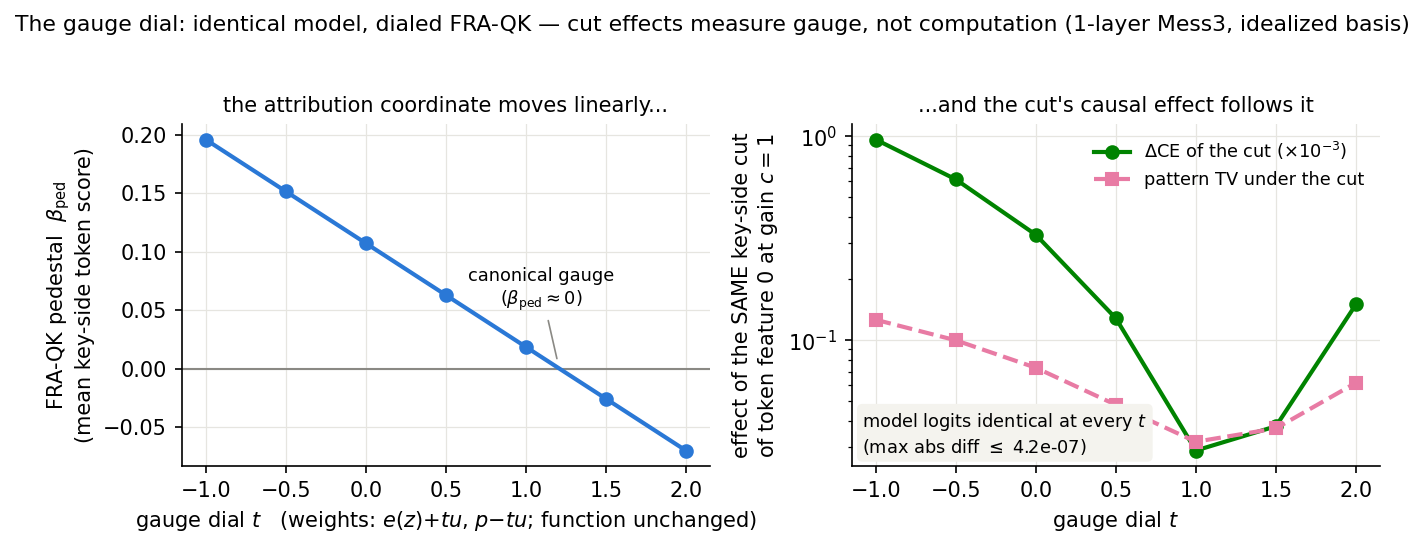
\includegraphics[width=0.95\textwidth]{../figures/gauge_dial.png}
\caption{The gauge dial on the trained 1-layer Mess3 model. Left: the embedding re-split moves the FRA-QK pedestal linearly through zero while the model's function is bit-identical at every dial value. Right: the behavioral effect of the \emph{same} key-side FRA-QK cut follows the dialed coordinate, collapsing at the canonical gauge.}
\label{fig:gaugedial}
\end{figure}

\subsection{Where FRA-QK genuinely works: the four-context parallelogram}\label{sec:parallelogram}

The gauge theorem is conditional on the optimal pattern being token-independent, and that is a property of the \emph{data}. On induction data the condition fails, provably, and FRA-QK acquires a real handle --- this is the regime where FRA interventions beat steering baselines in earlier experiments (\texttt{fra\_win}: induction, in-context backdoors). The proof that lag-only patterns cannot do induction is a four-line argument worth internalizing.

The induction task: predict the successor of the most recent earlier occurrence of the current token. Fix two context positions $s_1 < s_2$, a query token A at the end, and fixed successor tokens X (after $s_1$) and Y (after $s_2$). Consider four contexts differing only in the tokens at $(s_1, s_2)$:
\begin{center}
\begin{tabular}{llll}
\toprule
context & tokens at $(s_1, s_2)$ & task demands & margin for X over Y \\
\midrule
$C_1$ & (A,\; B) & most recent A is at $s_1$ $\Rightarrow$ predict X & $g_1 \ge m$ \\
$C_2$ & (B,\; A) & most recent A is at $s_2$ $\Rightarrow$ predict Y & $g_2 \le -m$ \\
$C_3$ & (A,\; A) & most recent A is at $s_2$ $\Rightarrow$ predict Y & $g_3 \le -m$ \\
$C_4$ & (B,\; B) & A appears nowhere: no preference & forced: $g_4 \ge m$ \\
\bottomrule
\end{tabular}
\end{center}
For any lag-only pattern with per-key values, the head output is $a(d - s_1)\,\nu(\text{token at } s_1) + a(d - s_2)\,\nu(\text{token at } s_2) + (\text{terms common to all four})$. The position-wise token multisets of $\{C_1, C_2\}$ and $\{C_3, C_4\}$ coincide --- each has one A and one B at $s_1$, one A and one B at $s_2$ --- so the outputs obey the parallelogram identity $\cb^{(1)} + \cb^{(2)} = \cb^{(3)} + \cb^{(4)}$ exactly, and so do the X-versus-Y logit margins: $g_1 + g_2 = g_3 + g_4$. The task's first three demands then force $g_4 = g_1 + g_2 - g_3 \ge m$: the model must confidently predict X in the one context that contains no A at all, where the truth prefers neither. Every lag-only model pays a fixed cross-entropy penalty; the optimum must gate its scores on content ($\eta\,\ind[z_s = z_d]$ does the job); the feature$\times$feature mass acquires a loss-pinned, gauge-\emph{invariant} component; and cutting it moves behavior by $O(1)$.

So the boundary of FRA-QK's usefulness is a crisp data property: \textbf{does the task force the pattern to depend on content?} Induction: yes. Belief updating over a stationary HMM --- and, a fortiori, counting block tags: no. On the counting side there is a second, independent protection mechanism, which is the next section.

\section{Puzzle 1, part two: running averages protect themselves}\label{sec:protection}

The gauge theorem says FRA-QK cut coefficients are unpinned; it leaves open the possibility that a large-gain edit, whatever its provenance, might still damage the concept by brute pattern distortion. The experiment says no: at the interface where keys carry raw token tags, every FRA-QK cut at every gain leaves RF $\le 0.10$ while the \emph{grammar} collateral CF climbs to $0.30$. The concept is specifically protected, and the protection has a one-line mechanism.

\textbf{The concept content of a key is its running average --- and running averages barely differ between keys.} Recall Eq.~\eqref{eq:count}: the posterior mean after $s$ tokens is $(\alpha + n(s))/(10 + s + 1)$. Between key $s$ and query $d$ it can drift by at most
\begin{equation}\label{eq:drift}
    \big|\omhat_k(d) - \omhat_k(s)\big| \;\le\; \frac{d - s}{\kappa + d} \qquad (\kappa = 10 \text{ in the toy}),
\end{equation}
deterministically --- each new token moves a count-based average by at most one part in $\kappa + d$ --- and the typical (mean-square) drift is smaller still, of order $\sqrt{(d-s)/((\kappa+s)(\kappa+d))}$, by the martingale property of posterior means. You can see the drift shrinking directly in the worked sequence: $\omhat_1 = 0.611$ at $t = 16$, $0.78$ at $t = 64$, $0.83$ at $t = 128$ --- adjacent stretches of keys agree about the concept to a few percent, and ever more tightly as the sequence grows.

Now replay the slogan of Section~\ref{sec:softmax}: a score edit moves a readout only through the covariance of the edit with that readout's per-key values. For a concept readout, the per-key values are (affine in) the running averages $\omhat(s)$, which agree across the attended window up to the drift bound. \emph{Any} pattern edit, at \emph{any} gain, only reshuffles weight among keys that nearly agree --- approximate Invariance 2. Quantitatively, for any edit $\delta$ at gain $c$ with $E = c\,\osc(\delta)$,
\begin{equation}\label{eq:protection}
    \big|\Delta(\text{concept readout})\big| \;\le\; (e^{E} - 1)\;\kappa_\omega\, \frac{L_d}{\kappa + d}, \qquad L_d = \text{the pattern's mean lag},
\end{equation}
so a geometric attention window ($L_d$ bounded) gives $O(1/d)$ protection, and even a flat counting window gives $O(1/\sqrt d)$ typical protection. Grammar readouts enjoy no such shield: their per-key values are functions of the token identity itself, $\psi(z_s)$, which jumps at full spread $\Gamma$ between adjacent keys --- block tags flip between 0, 1, 2 constantly --- so pattern edits move grammar by $\Theta(\Gamma)$ with no decay in $d$.

\textbf{The predicted signature is an asymmetry, and the toy shows exactly it:}
\begin{itemize}
    \item Concept protected, grammar exposed: RF $\le 0.10$ across the entire FRA-QK grid, while CF reaches $0.30$. The cut damages the machinery it can reach (belief tracking within components) and misses the machinery it was aimed at.
    \item Protection tightens with position, exposure does not: for the key-side \texttt{omega\_top4} cut at $c = 1$, per-position concept damage falls $0.0075 \to 0.0018 \to 0.0006$ from early to mid to late positions (at $c = 2$: $0.028 \to 0.010 \to 0.0014$) --- a $13$--$20\times$ early-to-late drop --- while CF stays order-one throughout.
    \item The decay follows the predicted power law on the primary run, and fails to on the replication. The clean pattern's mean lag is bounded ($7.5 \to 10.5$): a geometric-type window, for which the theorem predicts MSE damage $\propto (\kappa + t)^{-2}$; the measured exponent at $c = 2$ is $-1.97$ (95\% CI $[-2.12, -1.79]$). On the independently trained \texttt{seed43} run, damage instead \emph{rises} with position at $c = 2$ (exponent $+0.42$) --- consistent with the bound (whose $(e^{E}-1)$ prefactor can grow with position, and which covers only the direct head-output channel in this 3-layer model) but a real limit on the simple exponent story: one run of two.
\end{itemize}

\begin{figure}[h]
\centering
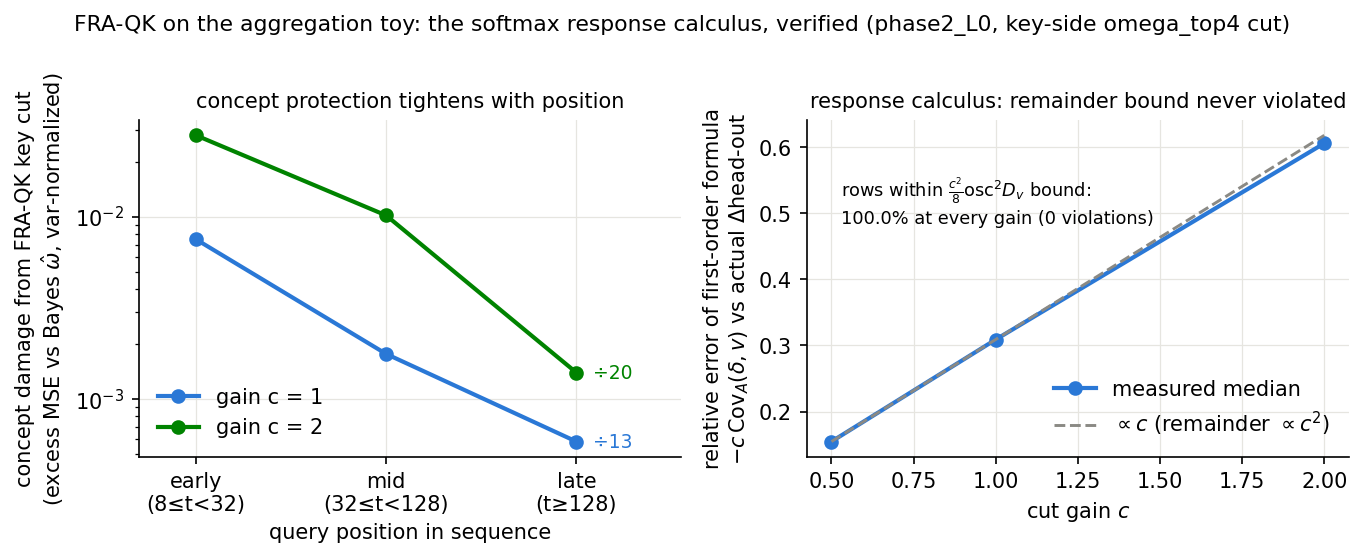
\includegraphics[width=0.95\textwidth]{../figures/qk_protection.png}
\caption{The QK side, verified on the mixture toy. Left: concept damage from the key-side FRA-QK cut falls $13$--$20\times$ from early to late positions --- aggregation protection tightening exactly as the drift bound prescribes. Right: the first-order covariance formula's error grows linearly in $c$ (remainder $\propto c^2$) and the $\tfrac{c^2}{8}\osc^2 D_v$ bound is never violated on any row.}
\label{fig:qkprotection}
\end{figure}

Putting the two parts of Puzzle 1 together: the feature$\times$feature attribution was gauge (Section~\ref{sec:gauge}), so cutting it had no reason to work; and even a cut with real oscillation lands on a readout whose keys agree (this section), so it had no way to work. Counting is doubly safe from routing surgery: \emph{the concept is carried by what is summed, never by who attends to whom.}

\section{Puzzle 2: the OV ``null'' is signal attenuation}\label{sec:ov}

\subsection{One number governs the whole gain sweep}

The FRA-OV cut subtracts $c$ times a \emph{fixed} vector field --- the $S$-content transported by this layer, computed once from the clean run --- so the intervened activation is exactly affine in $c$ by construction. Suppose for a moment that everything downstream of the hookpoint responds linearly too. Then the model's concept signal $m(t)$ (block-mass minus prior) can only be scaled:
\begin{equation}\label{eq:attenuation}
    m_c(t) = (1 - c\rho)\, m(t),
\end{equation}
where $\rho$ is the \emph{path share}: the fraction of the total concept flow into the output that passes through the cut path. Everything in the scoreboard's OV rows follows from this one line:
\begin{itemize}
    \item \textbf{Exact severing under-reaches.} At $c = 1$ the signal shrinks to $(1 - \rho)$ of itself. The toy's cut path carries a minority share, so severing it exactly leaves most of the concept flowing through parallel routes (the direct residual stream, other latents, later-layer re-aggregation): RF $0.06$.
    \item \textbf{The null is a calibrated cancellation.} The signal vanishes at $c^* = 1/\rho$: past $c = 1$ the edit injects an \emph{anti-concept} signal down one path, tuned to cancel the concept arriving by all the others. With the sweep-fit effective share $\rho \approx 0.25$, $c^* \approx 4$ --- the observed null.
    \item \textbf{The metrics inherit the scaling.} Tracking $R^2$ falls as $R^2_{\mathrm{clean}} - (c\rho)^2$, and RF $\approx (c\rho)^2$ because cross-entropy is locally quadratic in signal scaling around calibration. Sanity check at $c = 1$: $(0.25)^2 = 0.0625$ against observed RF $0.062$.
    \item \textbf{Presence is untouched, necessarily.} Scaling the \emph{expressed} signal down one path changes nothing about the concept content sitting in the residual stream and the parallel paths; a probe that refits simply reads it there: $R^2 = 0.985$ at the null. And overdriving past $c^*$ turns the edit into an anti-concept steering vector --- at $c = 6$ the sequence's true dominant component is pushed \emph{below} its prior.
\end{itemize}

``Remove the concept'' has quietly become two different tasks. The gain-tuned null removes the concept's \emph{use} --- its expression in behavior --- by destructive interference. The concept's \emph{presence} --- its decodability from the activations --- is a different quantity, which no pattern or path edit touches.

\subsection{Predicting the sweep before running it}

The attenuation law is falsifiable in a strong form: $\rho$ is measurable from the \emph{clean model alone}, by a single finite difference --- inject an infinitesimal multiple of the cut direction, read the slope of the concept signal (the measurement moves by at most $10^{-4}$ across two orders of magnitude of the probe step). On checkpoint \texttt{phase2\_L0} this gives
\begin{equation*}
    \hat\rho = 0.1745 \qquad (\text{independent run \texttt{seed43}: } \hat\rho = 0.1320),
\end{equation*}
and carrying this single linearization to its exact second-order consequences (the linear response also has a component orthogonal to the concept signal --- collateral that damages tracking without removing use --- plus a clean-residual cross term; both computable ex ante, still with no intervention data) predicts the whole sweep. Against the observed one:

\begin{center}
\begin{tabular}{crrrr}
\toprule
gain $c$ & RF predicted & RF observed & track $R^2$ predicted & track $R^2$ observed \\
\midrule
$0.5$ & $0.019$ & $0.019$ & $+0.977$ & $+0.977$ \\
$1.0$ & $0.061$ & $0.062$ & $+0.943$ & $+0.941$ \\
$1.5$ & $0.126$ & $0.126$ & $+0.889$ & $+0.881$ \\
$2.0$ & $0.214$ & $0.215$ & $+0.815$ & $+0.795$ \\
\bottomrule
\end{tabular}
\end{center}

Through $c \le 2$ the prediction is essentially exact --- third-decimal agreement in RF --- from one derivative of the clean model. The predicted null is $c^* = 4.91$ against the observed $4.00$ (\texttt{seed43}: $5.90$ vs $4.59$). The $\sim 20\%$ gap is itself measured rather than mysterious: the downstream stack (an MLP, another attention layer, the softmax) bends along the injection ray at large $c$, and the effective secant share grows from $0.18$ at $c = 1$ to $0.23$ at $c = 6$ ($31\%$ relative nonlinearity at $c = 4$) --- precisely the linearity assumption failing by a fifth, where the theory says the failure must show up.

The linearization even predicts the null's fine structure before looking. The path share rises with position ($\hat\rho = 0.132$ early, $0.171$ mid, $0.182$ late), so a single aggregate gain must under-cancel early positions and over-cancel late ones --- and the observed null indeed balances a $+0.11$ residual tracking early against $-0.09$ anti-tracking late. The ``null'' is an average of signed miscalibrations, and drifts off null on inputs whose signal strength differs from the calibration set (near-pure sequences get pushed anti-concept). A calibrated equilibrium, with the calibration visible.

\begin{figure}[h]
\centering
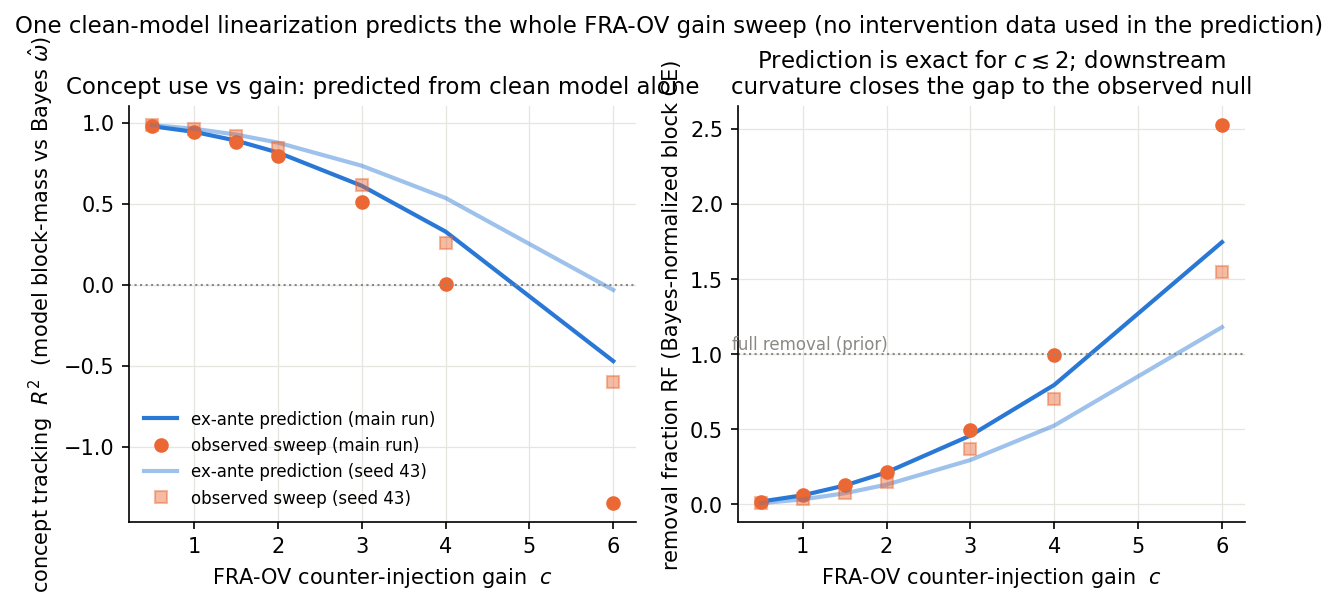
\includegraphics[width=0.9\textwidth]{../figures/attenuation_prediction.png}
\caption{Ex-ante attenuation predictions (from one finite difference on the clean model; no intervention data) against the observed FRA-OV gain sweep, for both independently trained runs. The refined-linear curves track the observations essentially exactly through $c \le 2$; the growing gap beyond is measured downstream curvature.}
\label{fig:attenuation}
\end{figure}

The one-layer Phase A model shows the same structure with the belief geometry exposed. Its per-token OV vectors align with the predicted belief displacements $\Bb(\pib\Tb^{|z} - \pib)$ at $\cos = 0.91$--$0.93$ (position-stable to $\cos > 0.998$), its attention-output probe prefers the constrained update over full Bayes ($R^2 = 0.818$ vs $0.766$), and the SAE-basis FRA decomposition of scores and attention output is exact to $2\cdot10^{-6}$ --- the attribution objects are the theory's objects. The interventions then reproduce the asymmetry at matched features: FRA-QK cuts of the two token latents at $c = 1$ move eval CE by at most $+0.0006$ ($5\%$ of the $0.012$-nat information window, growing superlinearly, $\approx 2.5\times$ per gain doubling), while FRA-OV severing of the \emph{same latents} at $c = 1$ costs $+0.0092$ --- $77\%$ of the window, a sixteenfold gap, with over-removal beyond severing ($c = 4$: $12.8\times$ the window). Content transported through the pattern is causally live; the pattern's token-resolved bookkeeping is not.

\subsection{The use/presence trichotomy}

The three intervention families now line up as three different operations on three different objects:

\begin{center}
\begin{tabular}{p{0.24\textwidth}p{0.34\textwidth}p{0.32\textwidth}}
\toprule
family & what it does to an aggregated concept & evidence \\
\midrule
\textbf{pattern edits} (FRA-QK, any set, side, gain) & reshuffle weight among keys that agree; use protected by drift, presence untouched; grammar pays $\Theta(\Gamma)$ & RF $\le 0.10$, CF up to $0.30$, presence $0.99$ \\
\textbf{path-content edits} (FRA-OV at gain $c$) & scale the expressed signal by $(1 - c\rho)$ along one path; use nulled at $c^* = 1/\rho$, presence untouched & RF $0.99$ at $c \approx 4$, presence $0.985$ \\
\textbf{content edits} (SAE cuts at the hookpoint) & remove the aggregate content itself where it fires: the only family that reduces presence & RF $0.86$, presence $0.99 \to 0.49$ \\
\bottomrule
\end{tabular}
\end{center}

Even the third family has a wall. The concept here is an aggregate statistic \emph{of the content the grammar needs}: $\omhat$ counts block tags, and belief updating must route each symbol's history to the right component using those same tags. A particle-filter computation of the ideal frontier gives the toy's \emph{entanglement tax}: an observer carrying zero $\omega$-information achieves within-block CE $0.845$ at best, against $0.7785$ with full information --- an irreducible $20.8\%$ of the grammar range that \emph{any} method must pay for full presence removal. Behavioral evals certify none of this: the $c \approx 4$ model passes every on-distribution behavioral test of concept use while carrying the concept at $R^2 = 0.995$. The audit that catches it is a presence probe, and the operative lesson of the whole toy is: \textbf{audit presence, not behavior.}

\section{One dial between the two regimes}\label{sec:dial}

Sections~\ref{sec:gauge}--\ref{sec:ov} describe two seemingly different worlds: an \emph{association} world (induction: content-gated patterns, FRA-QK has an $O(1)$ handle) and an \emph{aggregation} world (mixture counting: flat token-independent patterns, FRA-QK inert, FRA-OV = attenuation). One dial connects them: the spectral gap of the data process.

A hidden chain's transition operator has eigenvalues; the stationary eigenvalue $1$ carries what never decays, and eigenvalues $\lambda < 1$ carry evidence with memory horizon $\sim 1/(1-\lambda)$. The mixture concept is precisely extra eigenvalue-$1$ structure: the per-sequence label $\omega$ never changes, so the joint hidden process (mixture label $\otimes$ within-component state) has eigenvalue $1$ with multiplicity 3, and the concept subspace \emph{is} that eigenspace. The grammar lives in the $\lambda < 1$ modes. Aggregation is the $\lambda \to 1$ corner of the same framework, and the optimal attention profile interpolates continuously: solving the one-layer theory for a mode at eigenvalue $\lambda$ gives an optimal geometric window with rate $\eta(\lambda)$ obeying, as $\lambda \to 1$,
\begin{equation}\label{eq:flattening}
    1 - \eta \;\simeq\; \sqrt{\tfrac{2m}{\varphi}}\;\sqrt{1 - \lambda}
    \qquad\Longrightarrow\qquad
    \text{window } \frac{1}{1-\eta} \;\propto\; \frac{1}{\sqrt{1 - \lambda}} .
\end{equation}
The closed form matches direct numerical optimization to six decimal places across $\lambda \in [0.5,\, 0.9999]$, a free 300-lag profile optimization recovers the geometric shape exactly, and the window grows from $1.4$ to $75$ over that range (Figure~\ref{fig:flattening}). In the strict limit the optimal profile is exactly flat: counting, recovered as a spectral limit.

\begin{figure}[h]
\centering
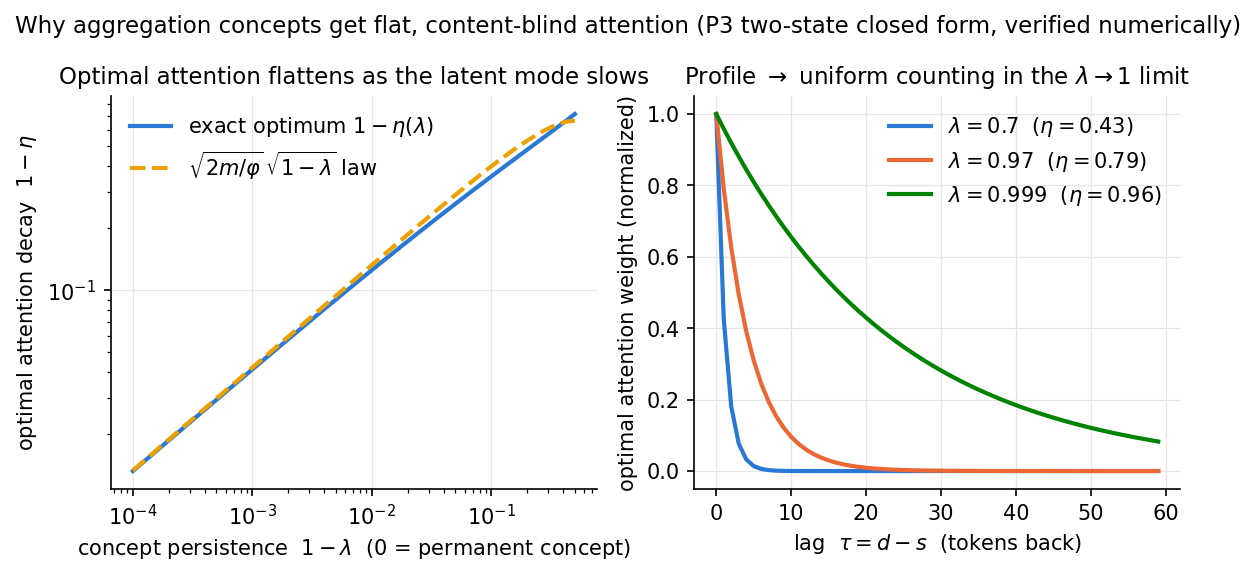
\includegraphics[width=0.85\textwidth]{../figures/flattening_law.png}
\caption{The flattening law. As the data eigenvalue $\lambda \to 1$, the optimal attention rate $\eta$ obeys $1 - \eta \propto \sqrt{1 - \lambda}$ and the effective window $1/(1-\eta)$ diverges: sharp associative patterns flatten into counting. Closed form against numerical optimization, agreement to six decimals; window $1.4 \to 75$ across $\lambda \in [0.5, 0.9999]$.}
\label{fig:flattening}
\end{figure}

Reading the dial from left to right gives the field guide:
\begin{itemize}
    \item \textbf{$\lambda$ well below $1$ (association regime).} Short memory, sharp patterns; tasks like induction force content gating (Section~\ref{sec:parallelogram}); the pattern is a causal carrier and FRA-QK edits it usefully; feature$\times$feature attribution has a loss-pinned component.
    \item \textbf{$\lambda \to 1$ (aggregation regime).} Long flat counting windows; the pattern is token-independent, so FRA-QK coefficients are gauge (Section~\ref{sec:gauge}); the concept rides in aggregated content whose keys agree, so all pattern edits are drift-bounded (Section~\ref{sec:protection}); FRA-OV acts as linear attenuation with a path-share null (Section~\ref{sec:ov}); and only content edits touch presence, up to the entanglement tax.
\end{itemize}
Every broad, slowly-varying in-context concept --- a topic, a persona, a per-document property estimated by accumulation --- is an aggregation-regime object. The toy's prediction for such concepts in real models is the scoreboard of Section~\ref{sec:puzzle}: spectral and attribution diagnostics will find mass; pattern surgery will find no handle; path severing will under-reach; gain-tuned cancellation will fake removal; and only content-level edits will move what a retrained probe sees.

\section{Honest limits}\label{sec:limits}

Four items bound how far the story above is proved, as opposed to measured.

\begin{enumerate}
    \item \textbf{The null gain is predicted to $\sim 20\%$, and the residue is measured curvature.} The ex-ante linearization matches the sweep to the third decimal through $c \le 2$, but $c^*$ sits at $4$--$6$, where the downstream map bends: the secant path share grows $0.18 \to 0.23$ over $c \in [1, 6]$. An exact ex-ante $c^*$ needs more than one linearization of the downstream stack; we report the one-derivative theory with its error measured, on both runs.
    \item \textbf{One idealized-basis prediction fails on the trained SAE, for a reason the theory names.} In the idealized basis, cutting the union of \emph{all} token features on the key side is a per-row constant --- exactly inert (Invariance 1). On the trained TopK SAE, the all-latents key cut is \emph{active}: its per-row score oscillation per unit of subtracted mass is $1.48\times$ that of the small \texttt{omega\_top4} set (the idealized theorem predicts a ratio far below $1$), and it does more at matched gain (RF $0.020$, CF $0.231$ at $c = 1$, versus $0.0023/0.045$). The mechanism: trained latents at this interface carry positional and aggregate content --- running counts correlate with position --- so the latent union subtracts part of the attention \emph{profile} itself, which no token-feature union does in the idealized basis. Per-feature statements (the covariance formula, the position scaling) transfer to the SAE basis; set-union statements are basis-sensitive.
    \item \textbf{Lag-only optimality for softmax/CE is a conjecture.} It is proved for the free-profile MSE surrogate, and trained softmax models measure as token-independent to precision --- but the CE case is open, and a model sitting slightly off the lag-only manifold has a small genuine content coupling, covered only by a measurable leak parameter. All gauge statements are exact \emph{given} token-independence.
    \item \textbf{Probe identifications are heuristic.} Reading the model's concept channel as a scaled posterior mean, and key values as functions of the block tag, is supported by probe $R^2$ rather than derived. The \emph{rates} in $d$ (the drift bounds, the position scaling) are independent of these identifications; the constants inherit them.
\end{enumerate}

Two habits the toy should install regardless: sweep intervention gains past $c = 1$ before declaring a null result (the operating point that mattered here sat outside the pre-registered grid); and when a behavioral null appears, retrain a probe before believing anything was removed.

\end{document}
